\section{Техническое задание}
\subsection{Основание для разработки}

Основанием для разработки является задание на выпускную квалификационную работу бакалавра "<Разработка веб-платформы для автоматизации бизнес-процессов управления персоналом компании">.

\subsection{Цель и назначение разработки}

Основной задачей выпускной квалификационной работы является разработка и внедрение веб-платформы для автоматизации бизнес-процессов управления персоналом компании.

Посредством внедрения веб-платформы планируется устранить существующие недостатки, связанные с децентрализованным и неэффективным управлением коммуникациями, задачами, календарными событиями и документооборотом.

Цель разработки включает следующие подцели:

\begin{itemize}
\item создание единой точки входа для всех внутренних сервисов компании;
\item интеграция различных бизнес-сервисов в рамках одной платформы;
\item обеспечение удобного доступа сотрудников к необходимым инструментам для работы;
\item оптимизация внутренних коммуникаций и процессов управления персоналом.
\end{itemize}

\subsection{Функциональные задачи}

Разрабатываемая веб-платформа включает в себя следующие модули:
\begin{itemize}
\item \textbf{Почта} — модуль корпоративной электронной почты для внутренней и внешней переписки;
\item \textbf{Контакты} — адресная книга с интеграцией к пользователям платформы;
\item \textbf{Проекты} — система постановки и контроля задач и проектов;
\item \textbf{Файлы} — облачное хранилище для совместного доступа к документам;
\item \textbf{Календарь} — планирование событий, встреч и мероприятий;
\item \textbf{Разговоры} — мессенджер для обмена сообщениями в реальном времени;
\item \textbf{ВКС} — модуль видеоконференцсвязи для онлайн-встреч;
\item \textbf{Настройки} — модуль настроек для смены или создания аватара, смены темы приложения;
\item \textbf{Панель управления} — страница с виджетами всех вышеперечисленных сервисов.
\end{itemize}

\subsection{Требования пользователя к интерфейсу web-сайта}

Платформа должна обеспечивать:
\begin{itemize}
    \item авторизацию;
    \item интуитивно понятную навигацию между модулями;
    \item адаптивный интерфейс для десктопных и мобильных устройств.
\end{itemize}

Композиция интерфейса пользователя представлена на рисунках ~\ref{templ:image1}, ~\ref{templ:image2}, ~\ref{templ:image3}, ~\ref{templ:image4}, ~\ref{templ:image5}, ~\ref{templ:image6}, ~\ref{templ:image7}, ~\ref{templ:image8}, ~\ref{templ:image9}.

\begin{figure}[ht]
	\centering
	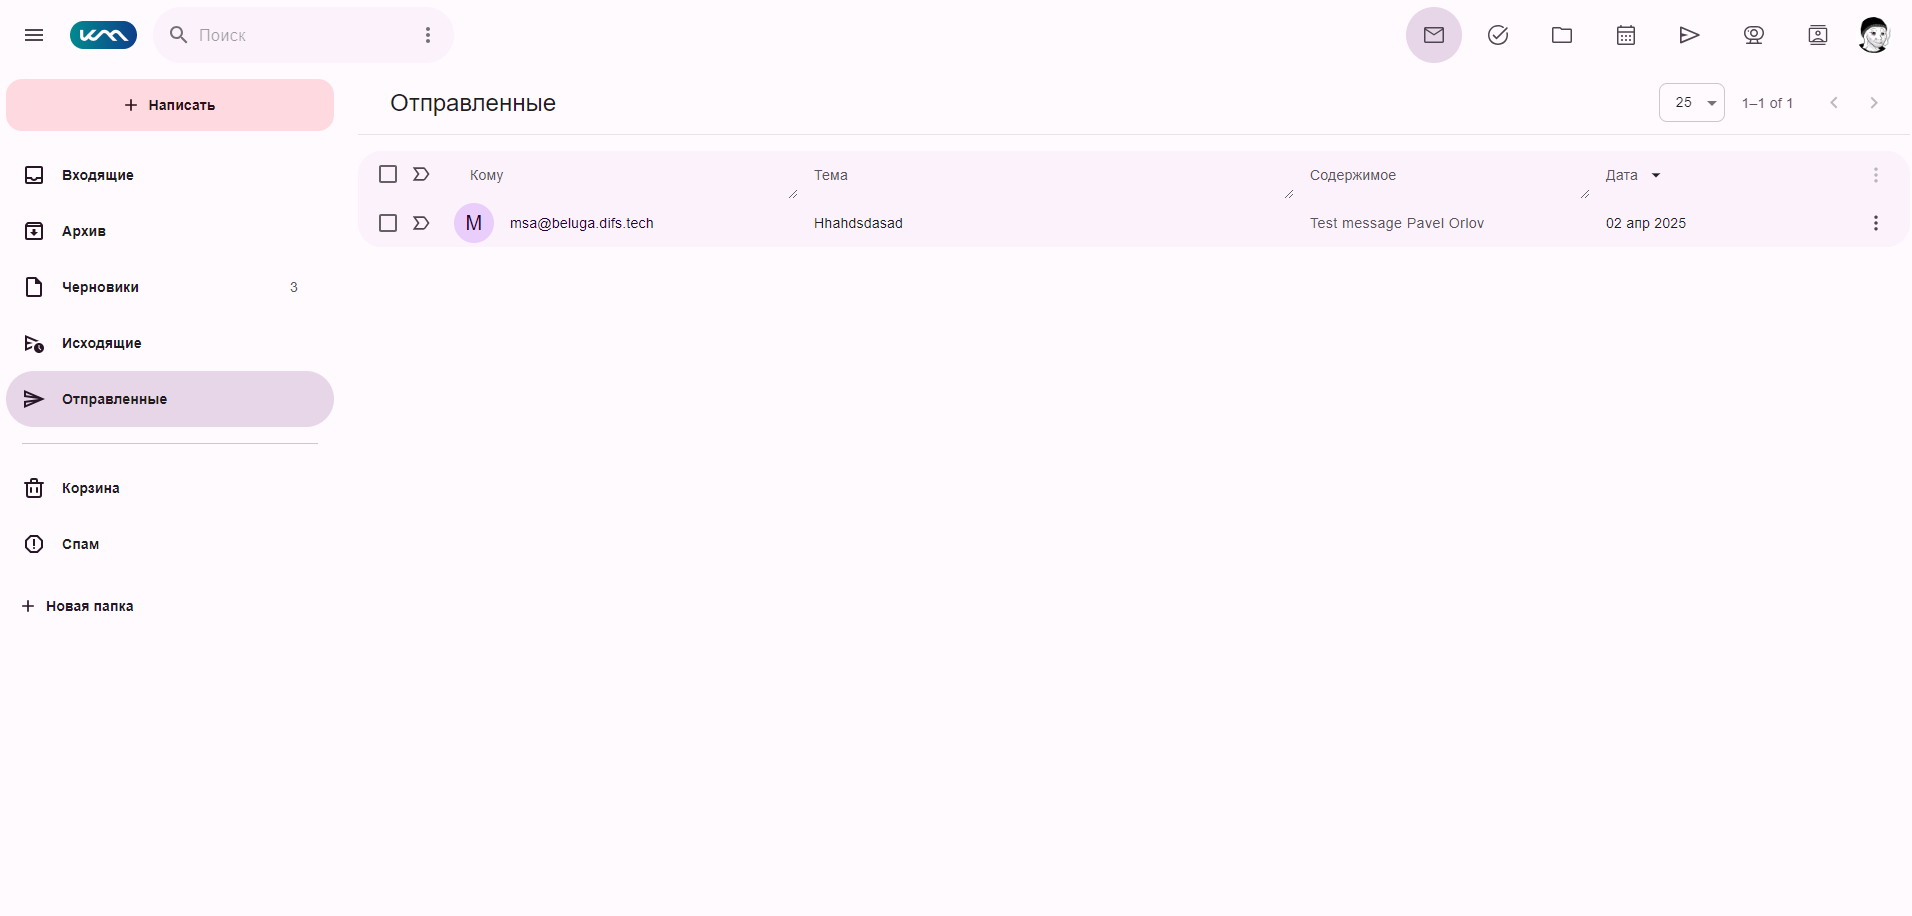
\includegraphics[width=1\linewidth]{images/почта}
	\caption{Композиция интерфейса сервиса <<Почта>>}
	\label{templ:image1}
\end{figure}

\begin{figure}[ht]
	\centering
	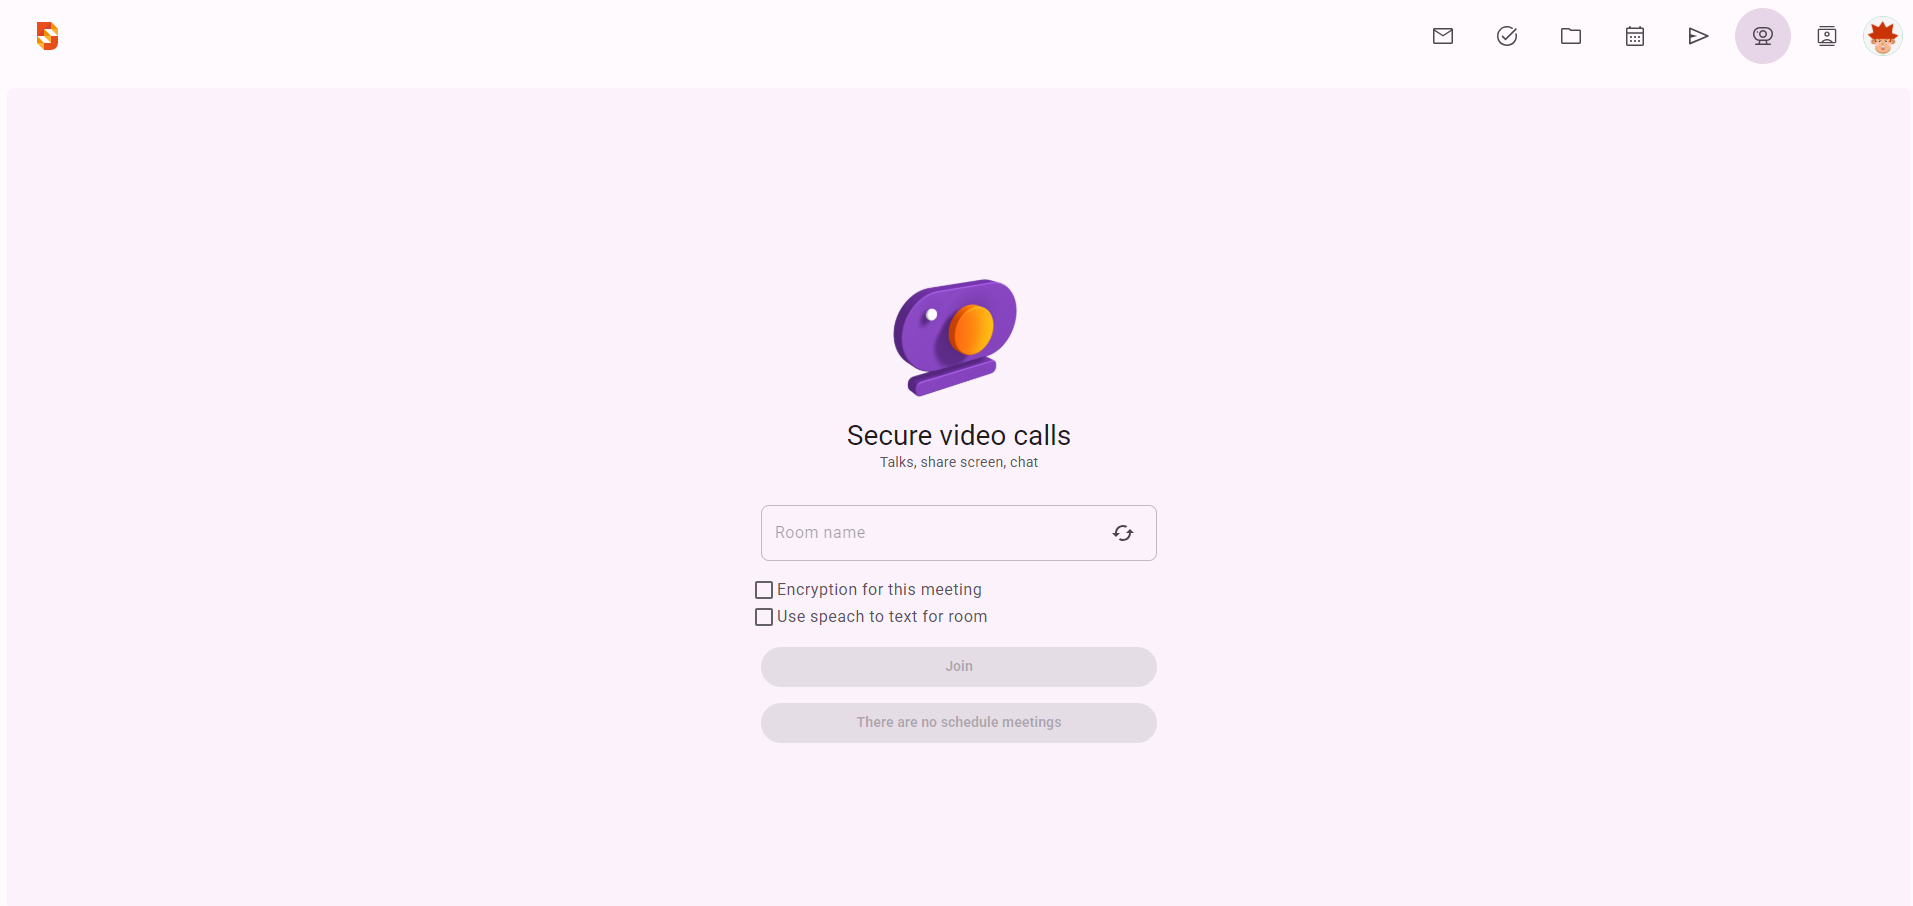
\includegraphics[width=1\linewidth]{images/вкс}
	\caption{Композиция интерфейса сервиса <<Видеоконференцсвязь>>}
	\label{templ:image2}
\end{figure}

\begin{figure}[ht]
	\centering
	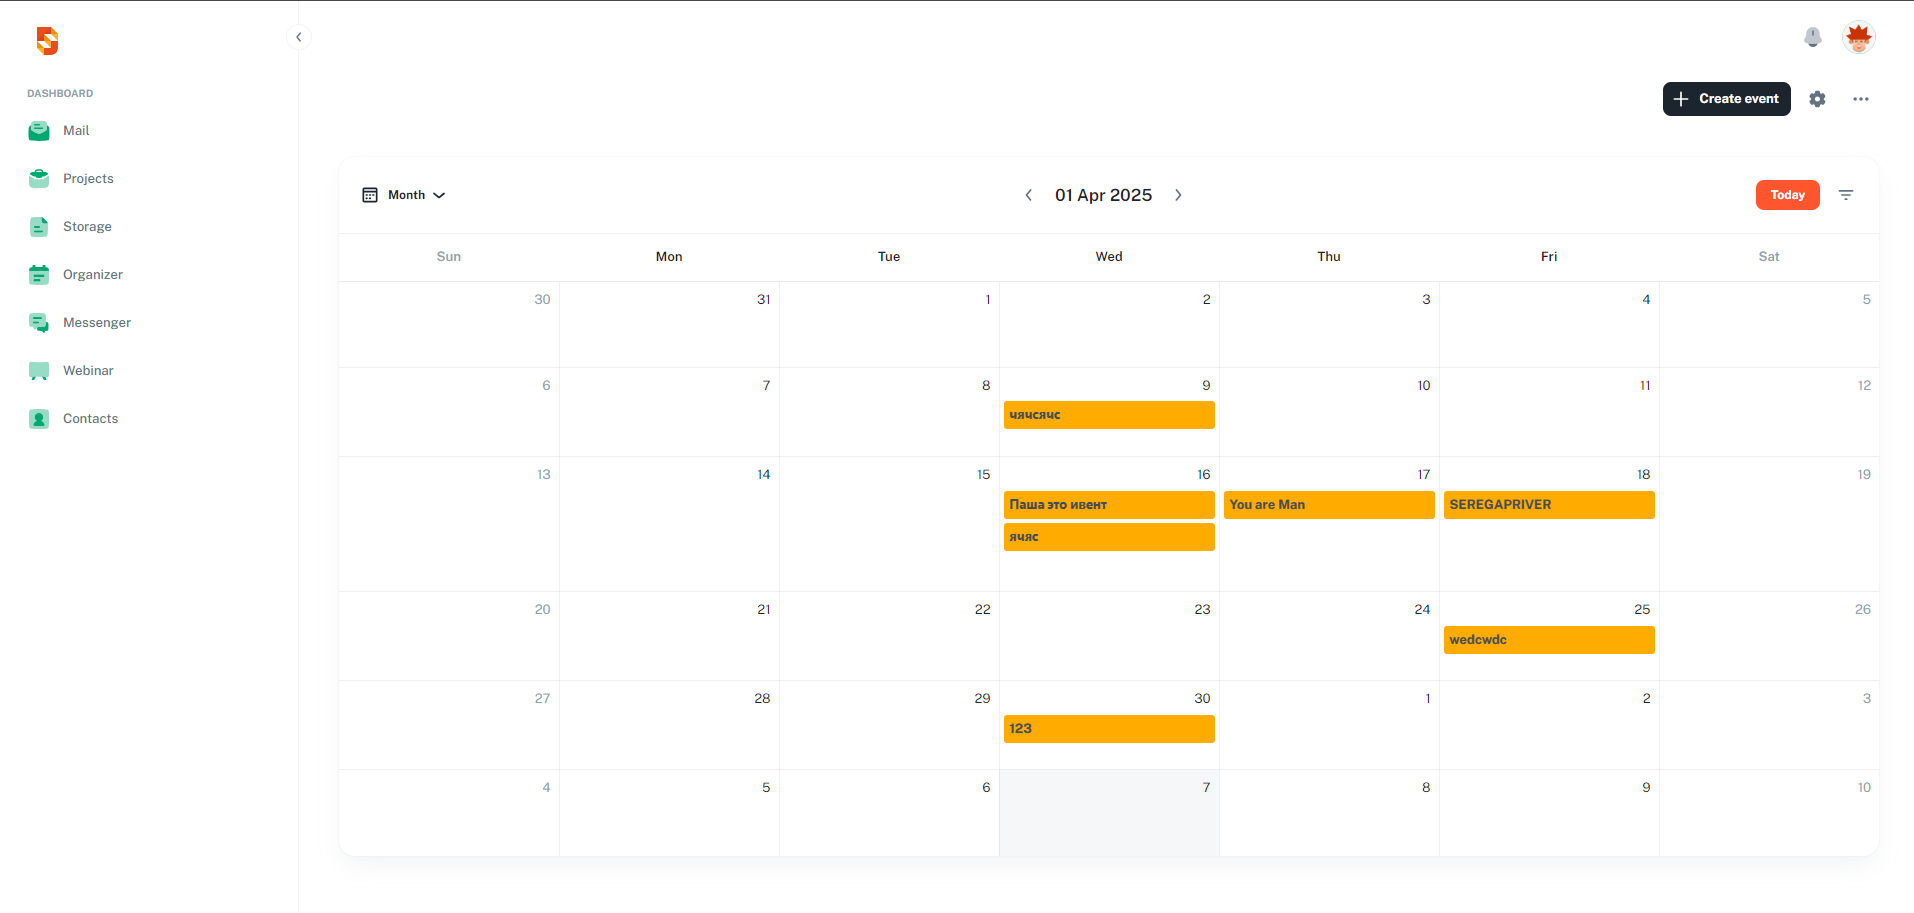
\includegraphics[width=1\linewidth]{images/календарь}
	\caption{Композиция интерфейса сервиса <<Календарь>>}
	\label{templ:image3}
\end{figure}

\begin{figure}[ht]
	\centering
	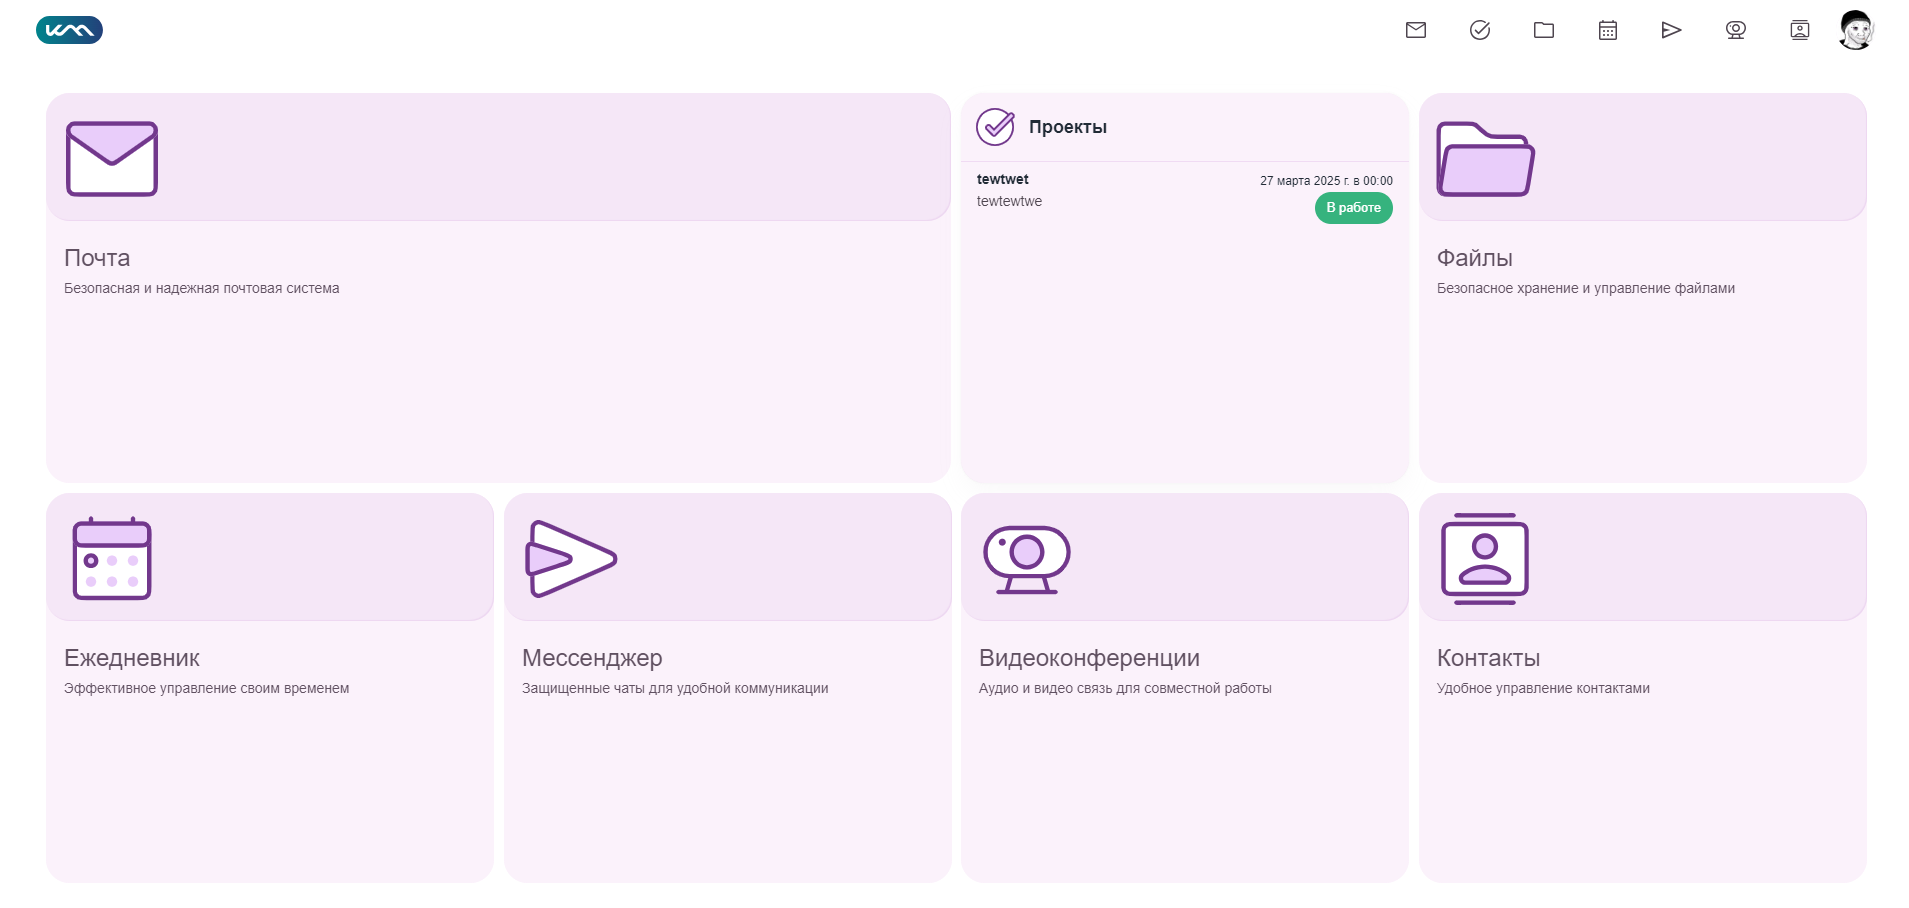
\includegraphics[width=1\linewidth]{images/дашборд}
	\caption{Композиция интерфейса сервиса <<Панель управления>>}
	\label{templ:image4}
\end{figure}

\begin{figure}[ht]
	\centering
	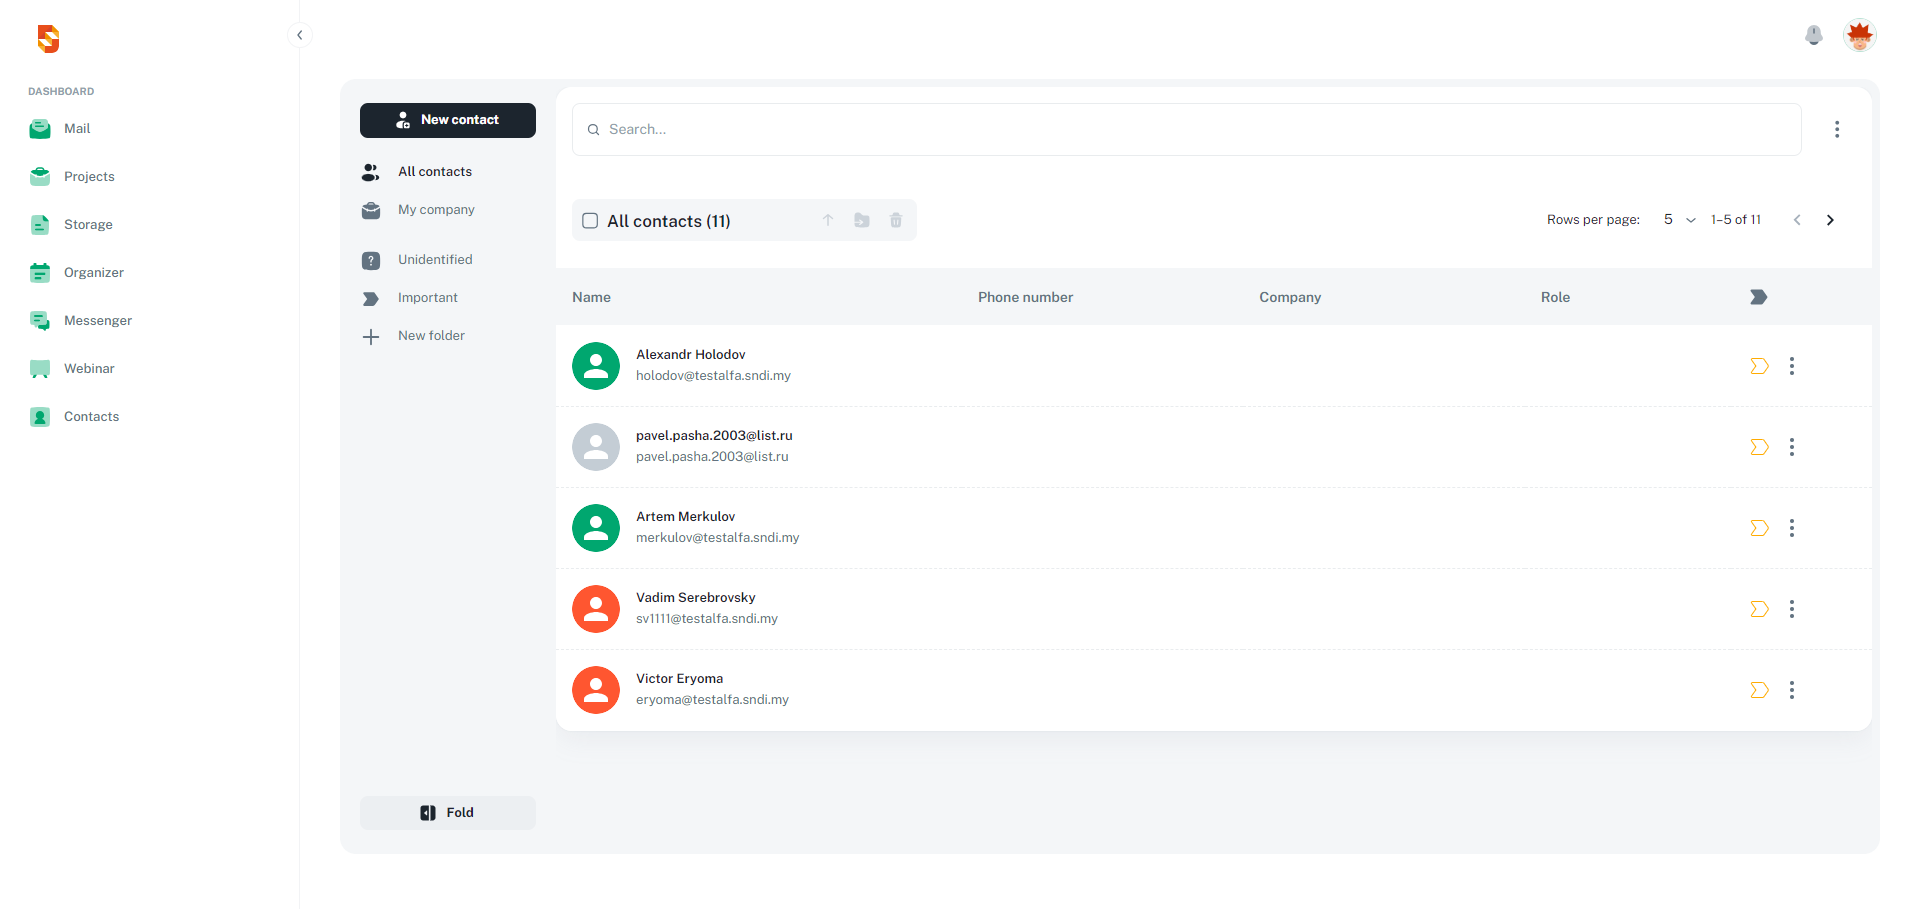
\includegraphics[width=1\linewidth]{images/контакты}
	\caption{Композиция интерфейса сервиса <<Контакты>>}
	\label{templ:image5}
\end{figure}

\begin{figure}[ht]
	\centering
	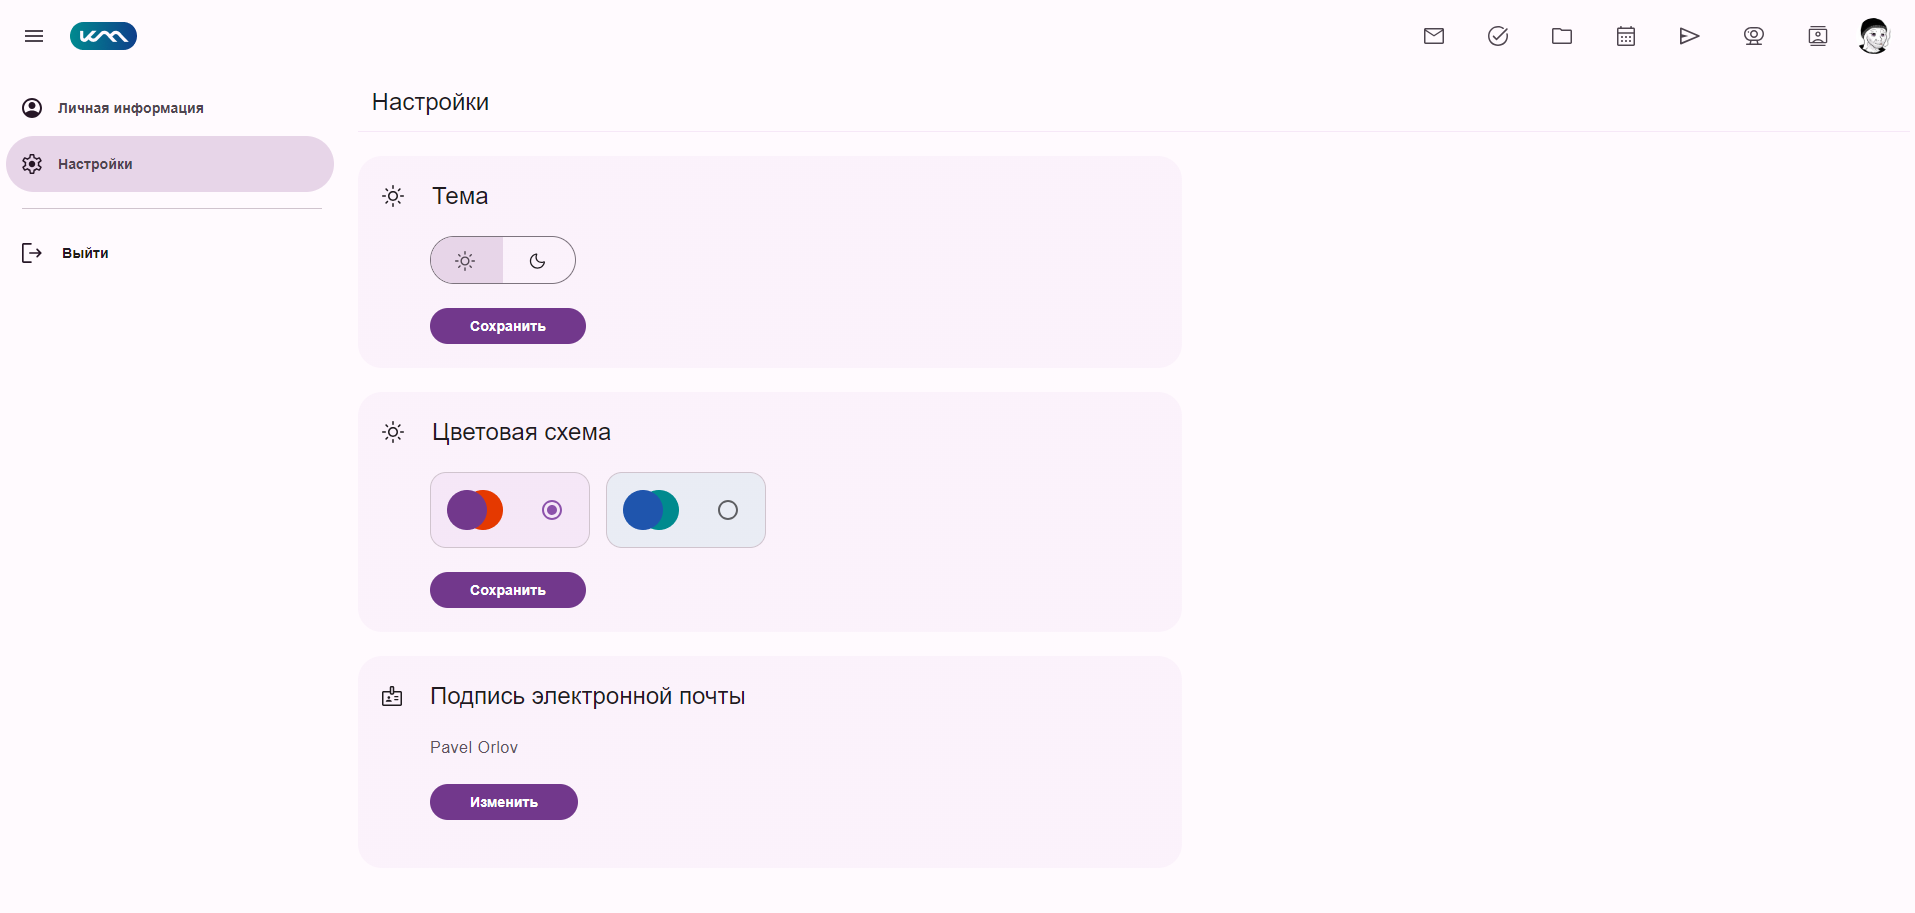
\includegraphics[width=1\linewidth]{images/настройки}
	\caption{Композиция интерфейса сервиса <<Настройки>>}
	\label{templ:image6}
\end{figure}

\begin{figure}[ht]
	\centering
	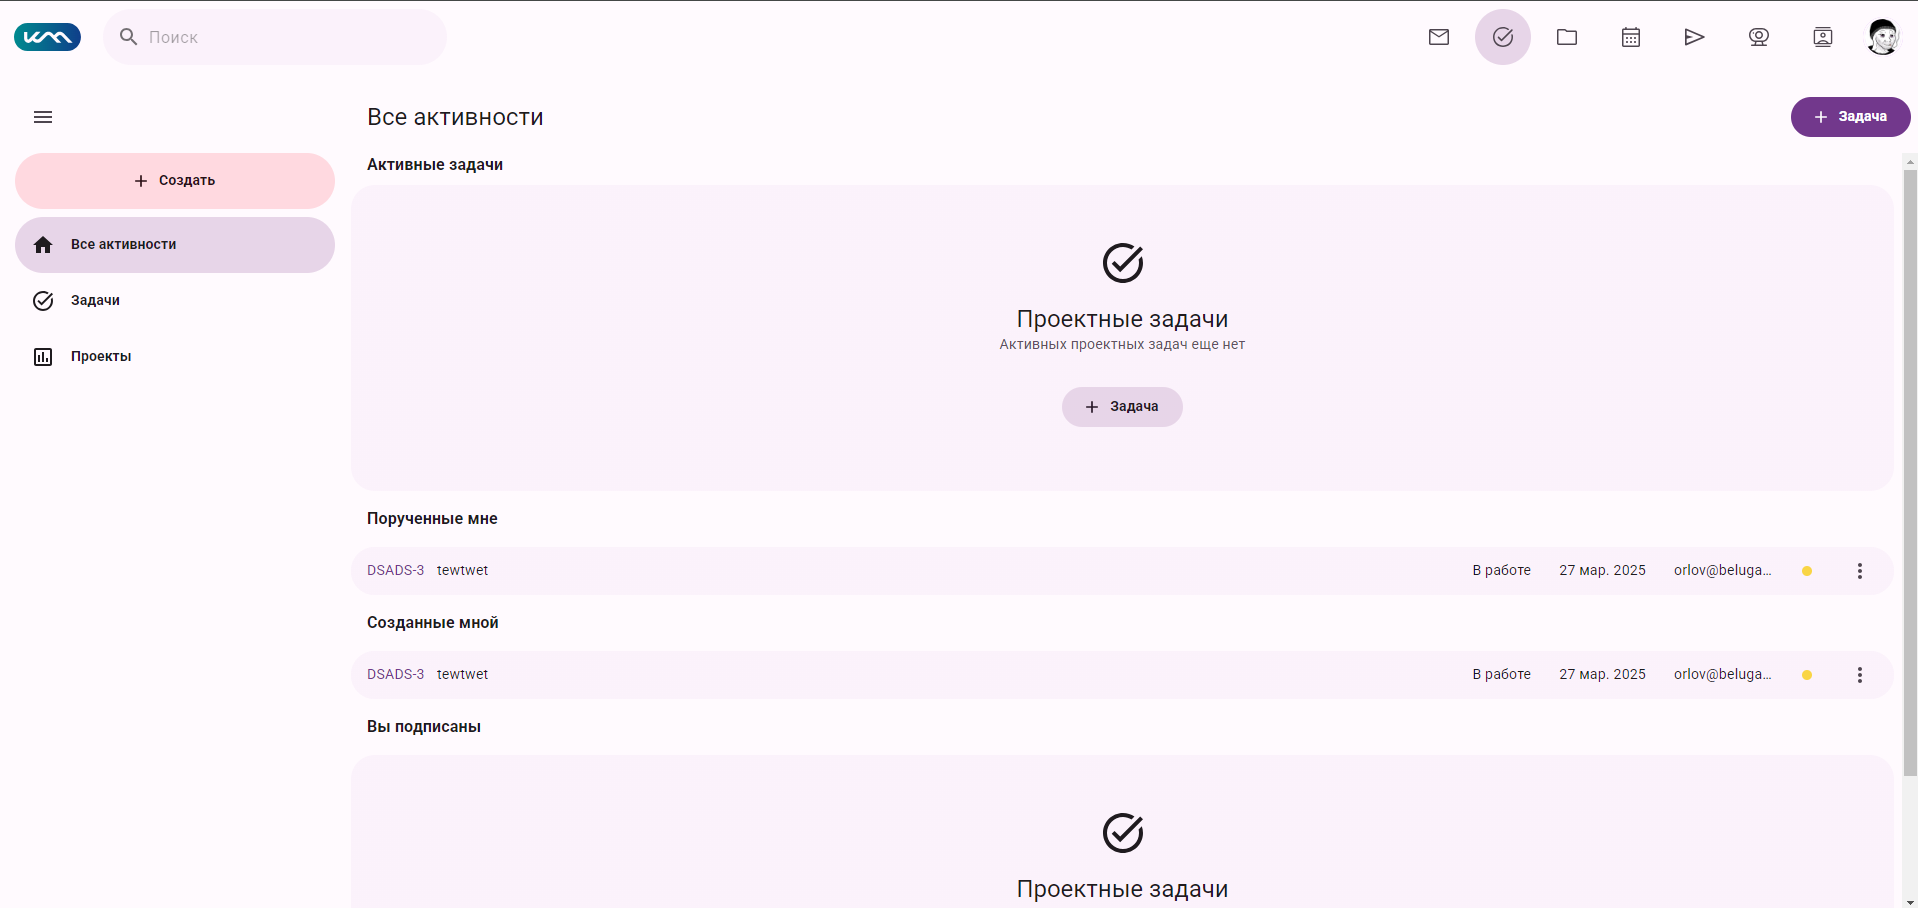
\includegraphics[width=1\linewidth]{images/проекты}
	\caption{Композиция интерфейса сервиса <<Проекты>>}
	\label{templ:image7}
\end{figure}


\begin{figure}[ht]
	\centering
	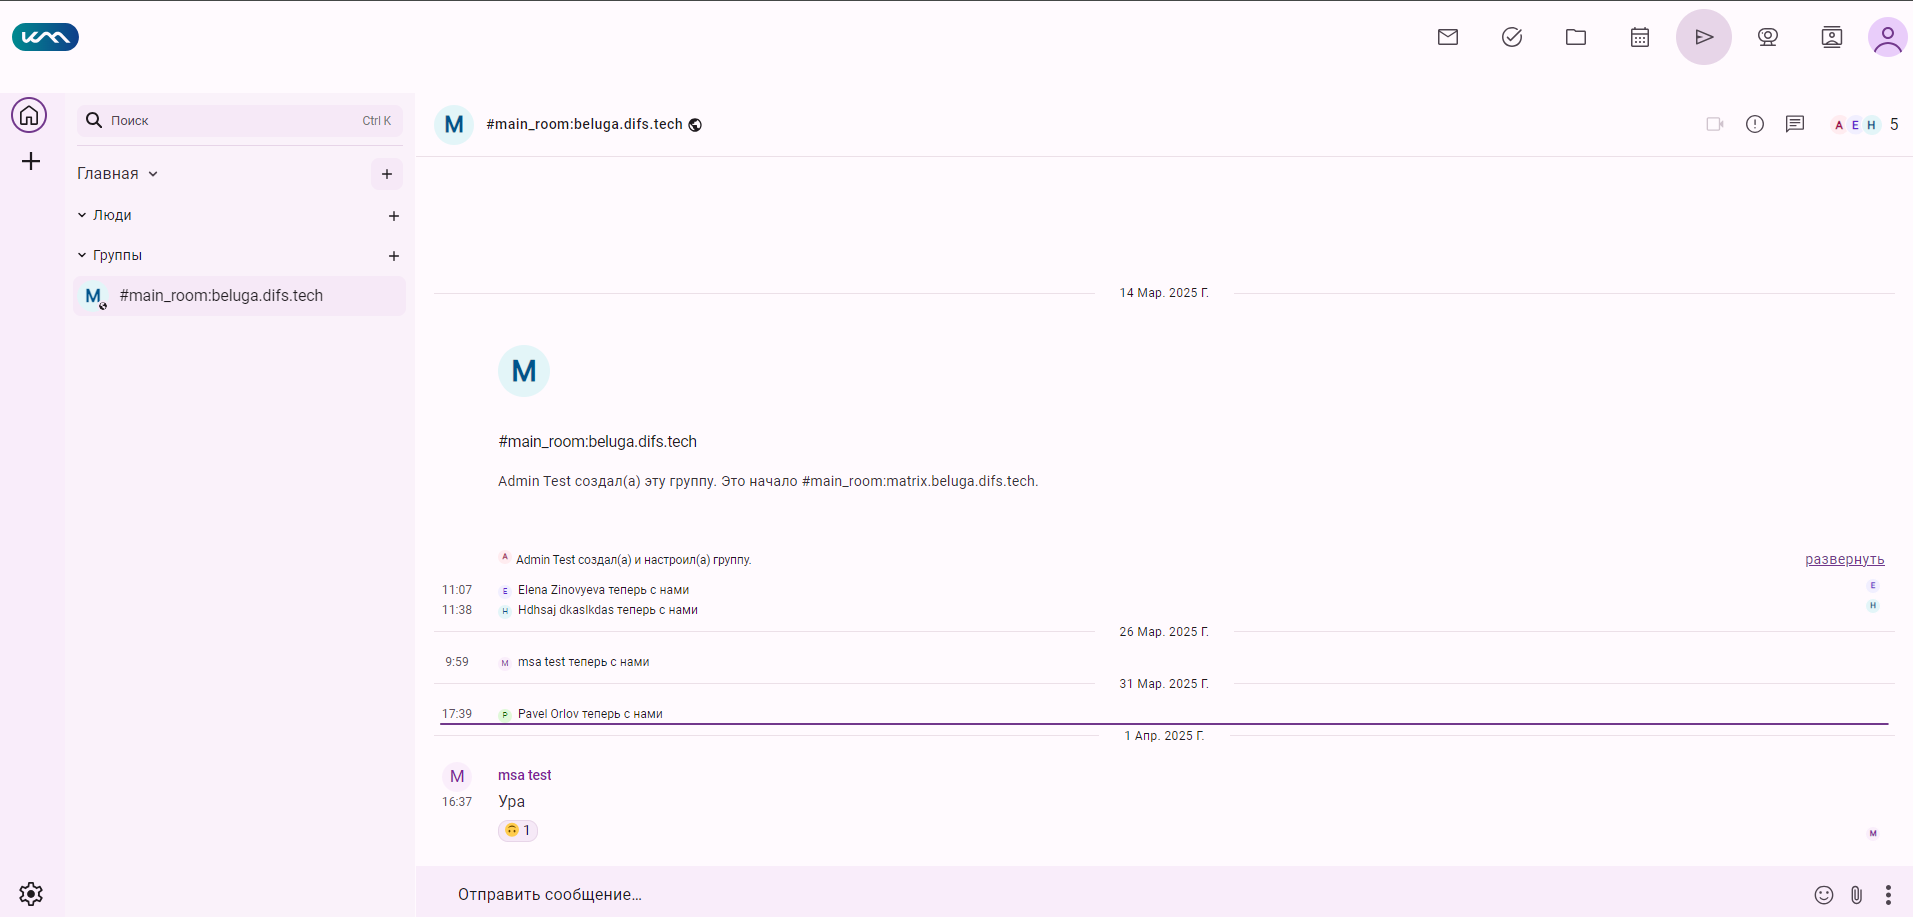
\includegraphics[width=1\linewidth]{images/разговоры}
	\caption{Композиция интерфейса сервиса <<Разговоры>>}
	\label{templ:image8}
\end{figure}


\begin{figure}[ht]
	\centering
	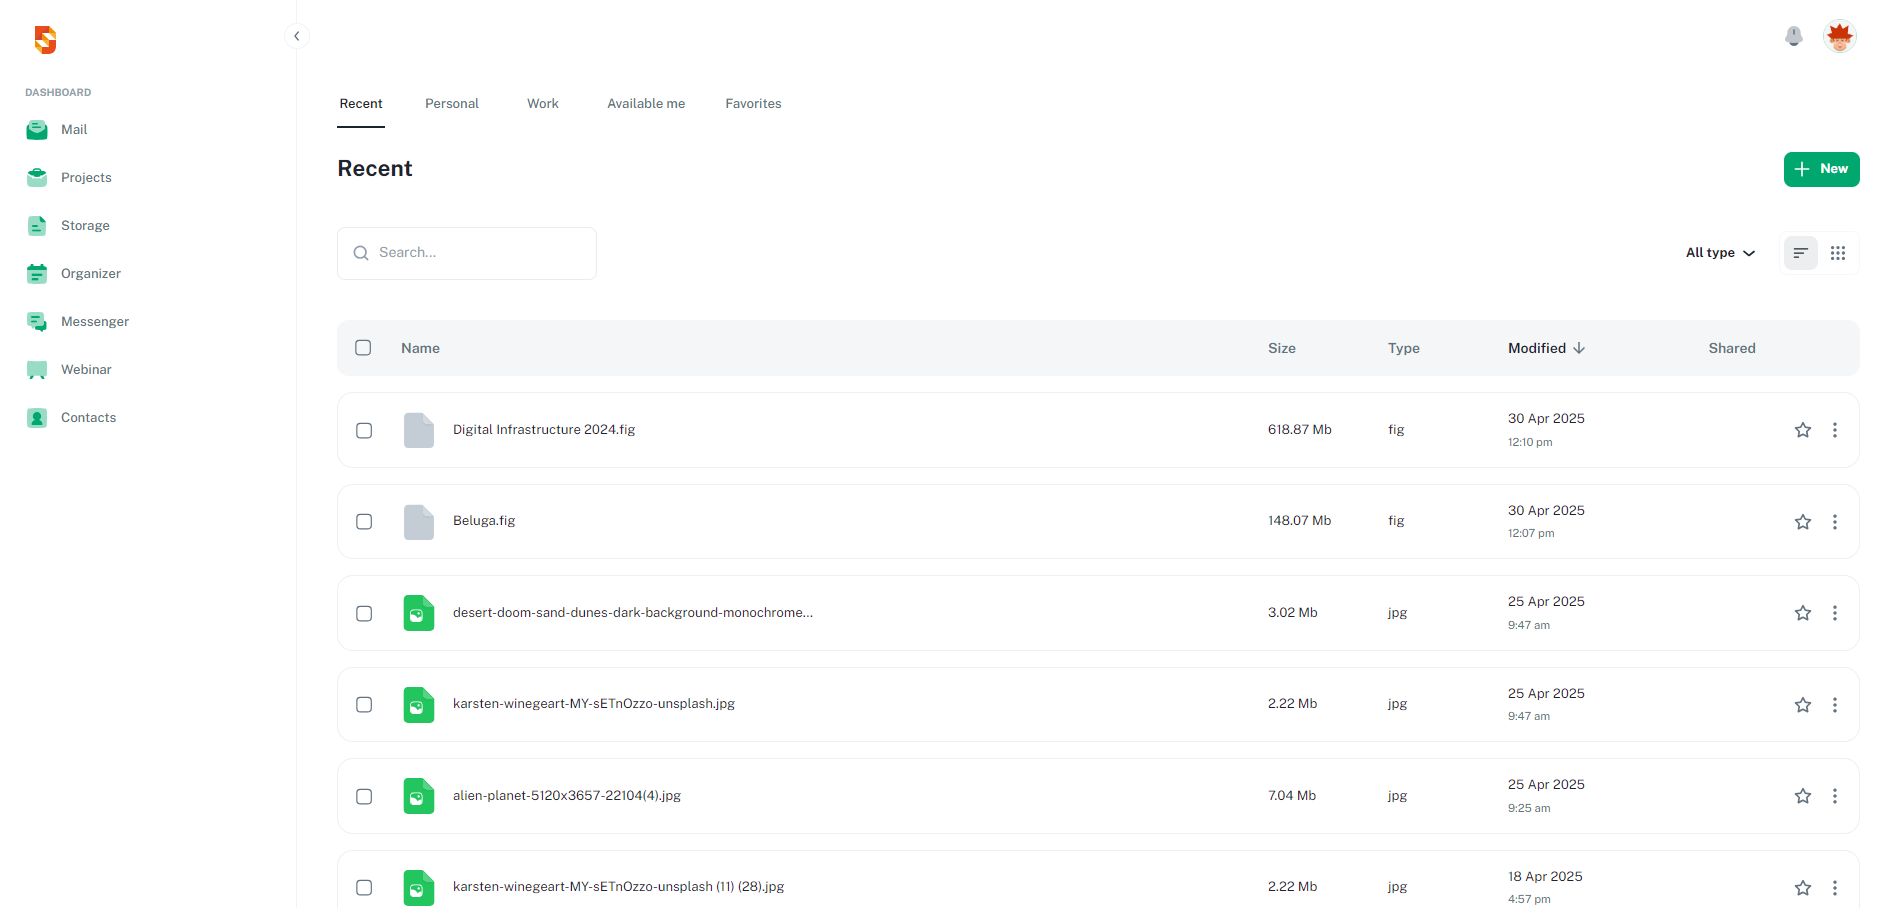
\includegraphics[width=1\linewidth]{images/файлы}
	\caption{Композиция интерфейса сервиса <<Файлы>>}
	\label{templ:image9}
\end{figure}

\clearpage
\subsection{Моделирование вариантов использования}

Для разработки платформы была построена UML-диаграмма вариантов использования, отражающая взаимодействие пользователей с системой.

Основные прецеденты системы:
\begin{enumerate}
\item Авторизация и выход из системы.
\item Отправка и получение сообщений в мессенджере.
\item Назначение задач и отслеживание их статуса.
\item Организация и участие в видеоконференциях.
\item Создание и просмотр календарных событий.
\item Управление файлами и документами.
\item Работа с корпоративной электронной почтой.
\item Персонализация панели управления.
\end{enumerate}

\subsection{Требования к оформлению документации}

Разработка программной документации и программного изделия должна производиться согласно ГОСТ 19.102–77 и ГОСТ 34.601–90. Единая система программной документации.
